\documentclass[tikz,border=14pt]{standalone}
% Shared look for every TikZ diagram. Load with \input{../../tools/tikz-style.tex}
\usepackage[T1]{fontenc}
\usepackage{lmodern}
\renewcommand{\sfdefault}{lmr}  % diagrams use the same serif as the text
\usetikzlibrary{arrows.meta, positioning, shapes.geometric, calc, fit, backgrounds}
\definecolor{cblue}{HTML}{4C78A8}
\definecolor{corange}{HTML}{F58518}
\definecolor{cgreen}{HTML}{54A24B}
\definecolor{cred}{HTML}{E45756}
\definecolor{cpurple}{HTML}{B279A2}
\definecolor{cgrey}{HTML}{6B6B6B}
\tikzset{
  every picture/.style={font=\sffamily, line width=1.2pt},
  box/.style={draw=#1, fill=#1!12, rounded corners=4pt, align=center, inner sep=7pt, minimum height=1.1cm},
  box/.default=cgrey,
  arrow/.style={-{Stealth[length=3mm]}, draw=cgrey, line width=1.4pt},
  title/.style={font=\sffamily\bfseries\Large},
  note/.style={font=\sffamily\small, text=cgrey, align=center},
}
\AtBeginDocument{\hyphenpenalty=10000 \exhyphenpenalty=10000}

\begin{document}
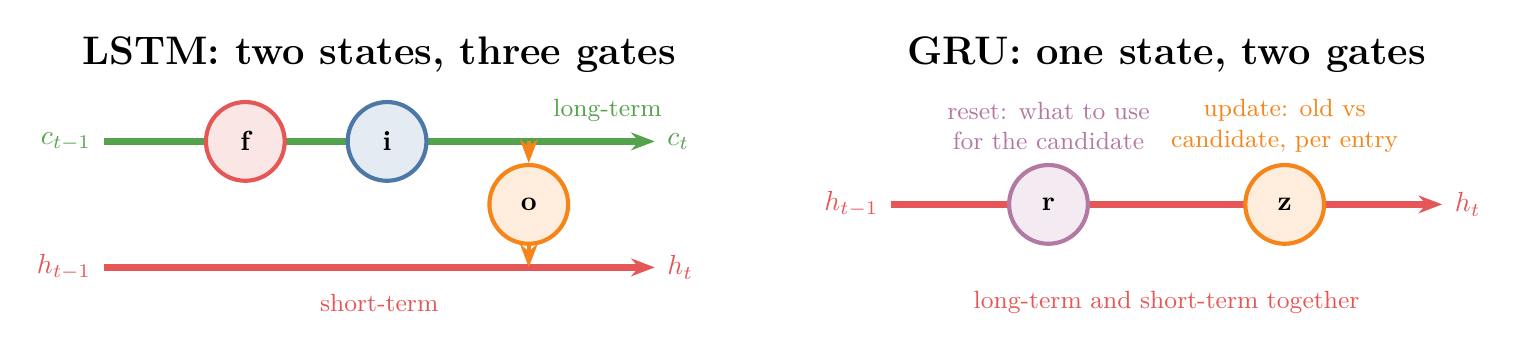
\begin{tikzpicture}[gate/.style={circle, draw=#1, fill=#1!15, line width=1.5pt, minimum size=1.0cm, font=\sffamily\bfseries}]
  % LSTM
  \node[title] at (3.5,3.3) {LSTM: two states, three gates};
  \draw[arrow, draw=cgreen, line width=2.5pt] (0,2.2) node[left, text=cgreen] {$c_{t-1}$} -- (7,2.2) node[right, text=cgreen] {$c_t$};
  \draw[arrow, draw=cred, line width=2.5pt] (0,0.6) node[left, text=cred] {$h_{t-1}$} -- (7,0.6) node[right, text=cred] {$h_t$};
  \node[gate=cred] at (1.8,2.2) {f};
  \node[gate=cblue] at (3.6,2.2) {i};
  \node[gate=corange] (o) at (5.4,1.4) {o};
  \draw[arrow, draw=corange] (5.4,2.2) -- (o); \draw[arrow, draw=corange] (o) -- (5.4,0.6);
  \node[note, text=cgreen] at (6.4,2.6) {long-term};
  \node[note, text=cred] at (3.5,0.15) {short-term};
  % GRU
  \node[title] at (13.5,3.3) {GRU: one state, two gates};
  \draw[arrow, draw=cred, line width=2.5pt] (10,1.4) node[left, text=cred] {$h_{t-1}$} -- (17,1.4) node[right, text=cred] {$h_t$};
  \node[gate=cpurple] at (12.0,1.4) {r};
  \node[gate=corange] at (15.0,1.4) {z};
  \node[note, text=cred] at (13.5,0.15) {long-term and short-term together};
  \node[note, text=cpurple] at (12.0,2.4) {reset: what to use\\for the candidate};
  \node[note, text=corange] at (15.0,2.4) {update: old vs\\candidate, per entry};
\end{tikzpicture}
\end{document}
